\documentclass[11pt, a4paper]{report}
\usepackage[a-1b]{pdfx} %PDF/A
\usepackage[utf8]{inputenc}
\usepackage[italian]{babel}
\usepackage{amsmath}
\usepackage{amsfonts}
\usepackage{hyperref} 
\usepackage{amssymb}
\usepackage{pdflscape}
\usepackage{chngcntr}
\usepackage{makeidx}
\usepackage{rotating}
\usepackage[utf8]{inputenc}
\usepackage{array}
\usepackage{subcaption}
\usepackage{datetime}
\usepackage{xcolor}
\usepackage{colortbl}
\usepackage{rotating}
\usepackage{tabto}
\usepackage{qrcode}
\usepackage{pstricks} %Per codice QR
\usepackage{pst-barcode} %Per codice QR
\usepackage{eurosym}
\usepackage{graphicx}
\usepackage{fancyhdr}
\usepackage{fancyvrb}
\usepackage{lmodern}
\usepackage{xurl} %per spezzare gli url inseriti con \url
\usepackage[left=2.5cm,right=2.5cm,top=3cm,bottom=3cm]{geometry}
\author{Alessandro Illuminati}
\hypersetup{
   % bookmarks=true,         % show bookmarks bar?
    %unicode=false,          % non-Latin characters in Acrobat’s bookmarks
   % pdftoolbar=true,        % show Acrobat’s toolbar?
   % pdfmenubar=true,        % show Acrobat’s menu?
   % pdffitwindow=false,     % window fit to page when opened
   % pdfstartview={FitH},    % fits the width of the page to the window
   % pdftitle={My title},    % title
   % pdfauthor={Author},     % author
   % pdfsubject={Subject},   % subject of the document
   % pdfcreator={Creator},   % creator of the document
   % pdfproducer={Producer}, % producer of the document
   % pdfkeywords={keyword1, key2, key3}, % list of keywords
   % pdfnewwindow=true,      % links in new PDF window
    colorlinks=true,       % false: boxed links; true: colored links
    linkcolor=black,          % color of internal links (change box color with linkbordercolor)
    %citecolor=green,        % color of links to bibliography
    %filecolor=magenta,      % color of file links
    urlcolor=blue           % color of external links
}


\newcommand\blfootnote[1]{%
  \begingroup
  \renewcommand\thefootnote{}\footnote{#1}%
  \addtocounter{footnote}{-1}%
  \endgroup
}

%______PREFAZIONE__________

\begin{document}
\newgeometry{left=2cm,right=2cm,top=2.65cm,bottom=2cm}
\begin{titlepage}
    \begin{center}
        
\includegraphics[scale=0.85]{immagini/UnivpmLogo.pdf} \\
        \vspace{5mm}

        {{\Large{\textbf{\large{UNIVERSITÀ POLITECNICA DELLE MARCHE}}}}} \\
        \vspace{3mm}
        \small{FACOLTÀ DI INGEGNERIA}
        \vspace{3.5mm}

        \rule[0.1cm]{17cm}{0.1mm}
        \rule[0.5cm]{17cm}{0.6mm}
        \\

        \large{{
                    Corso di Laurea triennale in \textit{Ingegneria Informatica e dell'Automazione}
                }}\\

    \end{center}

    \vspace{18mm}
    \begin{center}

        {
            \LARGE{
                \bf Implementazione di OpenVPN su router 4G per site-to-site vpn in ambiente CG-NAT
            }
        }\\

        \vspace{6mm}
        \Large{
            \textit{
                \#TODO Study and configuration of a site-to-site VPN in CG-NAT environment \#TODO
            }
        }\\

        \vspace{15mm}
    \end{center}
    \vspace{20mm}

    \noindent
    \begin{minipage}[t]{.49\textwidth}
        \flushleft

        {
            \large{Relatore:\\
                \vspace{1mm}
                \bf{Prof. Ennio Gambi}
            }\\

            \vspace{4.3mm}

            \large{Correlatore:\\
                \vspace{1mm}
                \bf{Ing. Adelmo De Santis}
            }

        }

    \end{minipage}
    %
    \hspace{1mm}
    %\hfill
    %
    \noindent
    \begin{minipage}[t]{.49\textwidth}
        \vspace{6.5mm}
        \flushright
        {\large{ Tesi di Laurea di:\\
                \vspace{1mm}
                \bf{Alessandro Illuminati}
            }\\
        }
        \vspace{2mm}
        \small{\textit{matricola} 1078466}
    \end{minipage}


    %\vspace{20mm}
    \vfill
    \begin{center}
        \rule[0.1cm]{17cm}{0.1mm}
        {
            \large{
                Anno accademico 2020-2021
            }
        }
    \end{center}
\end{titlepage}
\restoregeometry

\clearpage
\thispagestyle{empty}
\phantom{a}
\vfill
%\centering 
%\vfill
\newpage

%\input{contenuti/dedica}
%\clearpage
\thispagestyle{empty}
\phantom{a}
\vfill
%\centering 
%\vfill
\newpage

\pagenumbering{roman}
\clearpage
\phantom{a}
\vfill

\begin{center}
    \textbf{Prefazione}
\end{center}

\begin{flushleft}

    Nell'ambito del mio percorso universitario ho avuto modo di approfondire le tematiche relative al mondo delle reti e del networking, a tal proposito grazie alla possibilità offerta dal Dipartimento di Ingegneria dell'Informazione, dal Prof. Ennio Gambi e dall'Ing. Adelmo De Santis ho conseguito con successo la certificazione "\textit{HUAWEI HCIA Routing and Switching}".\\
    Successivamente, grazie alle competenze acquisite, ho collaborato con alcuni miei colleghi
    per progettare e realizzare una implementazione di una VPN site-to-site attraverso una connessione radiomobile per conto dell'azienda Esse-ti S.r.l.\\
    In questo elaborato verranno esposte le principali fasi del
    progetto realizzato, ponendo un particolare focus sulle problematiche iniziali affrontate e all'architettura di rete nel cui ambito è stata realizzata la comunicazione tramite un canale sicuro.

\end{flushleft}

\vfill
\newpage

%___________INDICE_CAPITOLI__________

\tableofcontents %Indice capitoli
\newpage

%___________INDICE_FIGURE_______

\listoffigures
\begin{flushleft}
  \blfootnote{
    \textit{Nella didascalia di ogni immagine vi è il link della pagina web da cui è stata presa, inoltre, sono citate anche accanto ai link nella sitografia.}
  }
  \\

\end{flushleft}
\newpage

%%___________INDICE_TABELLE__(Non serve)_____________________
%\listoftables
%\newpage


%___________CONTENUTI_______________________________
\pagenumbering{arabic}
\setcounter{page}{1} %Set numero di pagina


\chapter{Introduzione}
\setlength{\parskip}{1em}
\setlength{\parindent}{0em}
\renewcommand{\baselinestretch}{1.15}
\section{Scopo e analisi del progetto} \label{Scopo_e_analisi_del_progetto}

Nell'ambito di una convenzione stipulata con il Dipartimento di Ingengeria dell'Informazione, l'azienda \textbf{Esse-ti S.r.l.} ha esposto il suo progetto di fornire ad un certo gruppo dei propri clienti un router 4G per permettere di raggiungere e controllare dispositivi domotici, cablati e non, esterni alla rete locale dell'utente.
Il gateway fornito al cliente risulta dotato di una batteria e di uno slot SIM  quindi in grado di connettersi a \textit{global internet} attraverso una connessione geografica radiomobile, in particolare mediante la connettività 4G garantita da un \textit{Internet Service Provider} nazionale. Questa caratteristica permettere ai dispositivi connessi al gateway di fruire di un accesso ad internet e della possibilità di gestire comunicazione vocali, con il vantaggio di essere indipendenti da eventuali guasti che possono occorrere all'alimentazione elettrica o alla connettività via cavo nel luogo d'installazione dell'apparato.\\
Il lavoro si è focalizzato sul rendere possibile una comunicazione sicura tra un calcolatore autorizzato del cliente, situato nella rete locale dello stesso, e un dispositivo installato in un'altra sede fisica connesso al gateway fornito, nonostante le reti dei grandi provider mobili adottino nella maggior parte dei casi l'uso del protocollo \textbf{CG-NAT}, che impedisce la comunicazione diretta tra i due \textit{end-point} della trasmissione.
Per realizzare questa particolare configurazione di rete è stato perciò necessario utilizzare un server esterno dotato di un indirizzo IP pubblico, appoggiandosi ad un servizio \textit{VPS} fornito in particolare dal provider \textbf{OVHCloud}. In seguito si è dovuto provvedere alla creazione di una connessione sicura per i dati nel trasito attraverso la rete pubblica dal calcolatore del cliente al cloud server e infine dallo stesso al device domotico finale.
Una volta ottenuto l'accesso all'istanza server remota, dopo una verifica delle caratteristiche computazionali e di compatibilità software della stessa, si è deciso di adottare la suite open-suorce \textbf{OpenVPN} per l'implementazione dei tunnel cifrati attraverso i quali instaurare la comunicazione; questo software, a configurazione conclusa, garantirà un canale virtualmente diretto tra i due \textit{end-point}, in altre parole essi risulteranno connessi ad una stessa rete locale.

Per la realizzazione e la verifica della configurazione richiesta, la problematica è stata schematizzata in una topologia di rete di test facendo le seguenti semplificazioni ed osservazioni:
\begin{itemize}
	\item Ogni cliente ha accesso ad un unico gateway remoto;
	\item Ogni gateway è caratterizzato da più interfaccie, una di queste è connessa a global internet tramite la tecnologia radiomobile;
	\item Le restanti interfaccie del gateway sono tutte caratterizzata da uno spazio degli indirizzi privato, in generale ad esse possono essere collegati diversi dispositivi;
	\item La connessione sicura dal calcolatore del cliente al server remoto sarà di facile configurazione tramite l'interfaccia grafica del software OpenVPN;
	\item Dovrà essere possibile raggiungere dall'elaboratore del cliente, con il comando di debug \textit{ping}, uno dei device connessi al gateway remoto, garantendo la bidirezionalità della comunicazione.
\end{itemize}
Di seguito (Figura \ref{fig:topologia_di_rete}) viene proposto lo schema di principio che permette di realizzare la comunicazione desiderata con i vincoli posti, adottando le tecniche già citate.
\vspace{5mm}
\begin{figure}[ht]
	\centering
	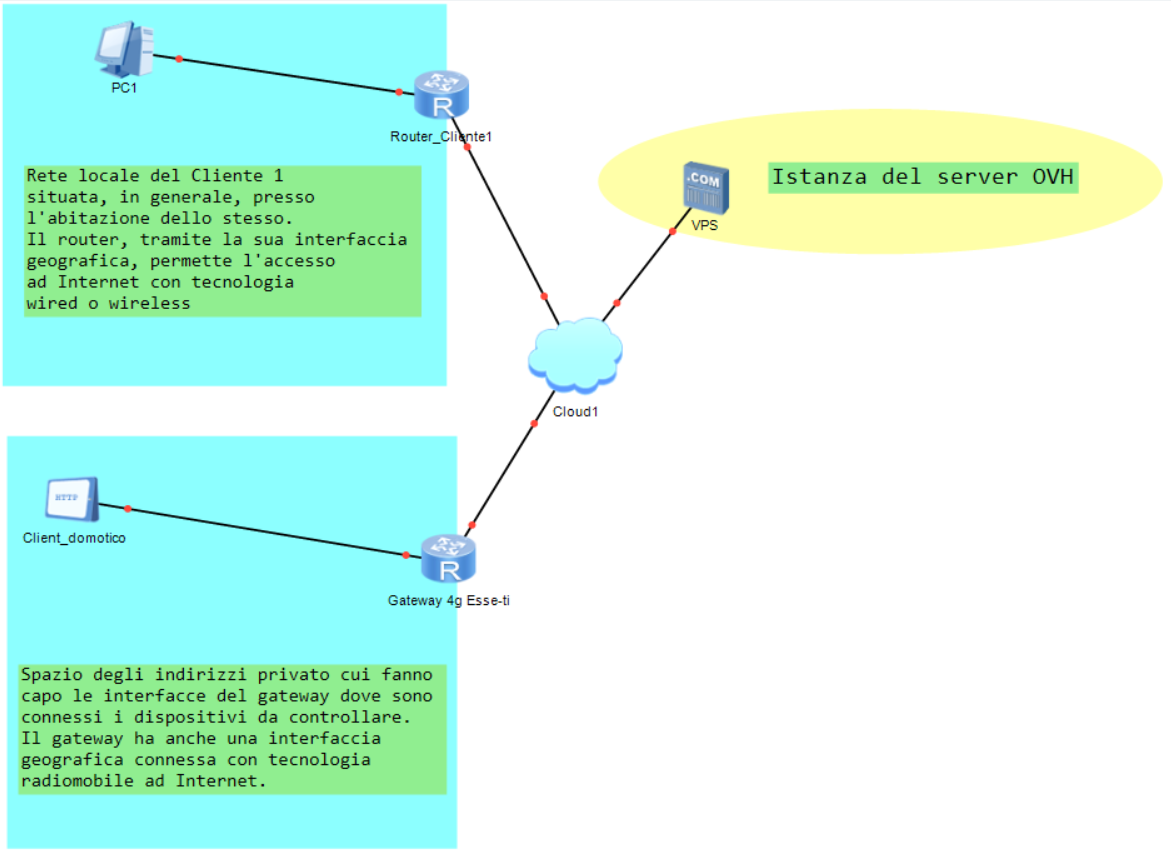
\includegraphics[width=1\textwidth]{immagini/topologia_di_rete_semplificata.png}
	\caption{Topologia di rete di principio adottata per la comunicazione}
	\label{fig:topologia_di_rete}
\end{figure}
\section{Generalità sui servizi VPS e caratteristiche del particolare servizio scelto }\label{caratteristiche_vps}

Per realizzare la comunicazione progettata si è evidenziata la necessità di un server remoto, che provveda a veicolare i dati tra i due \textit{end point} della comunicazione.
In particolare l'azienda ha richiesto un servizio che, seppur costoso, sia in grado di garantire un’alta affidabilità, bassa latenza e che in generale ponga pochi vincoli ad ulteriori e futuri sviluppi (quali ad esempio VNC o un servizio di desktop remoto), sia in termini di prestazioni offerte, sia in quanto a banda garantita.
Ad una prima analisi, ci sono 3 grandi player che offrono sul mercato servizi cloud altamente configurabili, potenti e granitici: \textit{Amazon AWS}, \textit{Microsoft Azure} e \textit{Google Cloud}. I prezzi proposti variano molto in base al servizio richiesto, abbiamo importi contenuti per macchine che lavorano a “trigger”, fino a cifre più importanti per macchine always-on che riservano staticamente delle precise risorse; inoltre è possibile anche configurare dei limiti di budget con i relativi avvisi.
In una successiva discussione si è deciso di usare un servizio più economico per le finalità di test preposte, e la scelta si è orientata su due provider in particolare, Aruba ed OVHCloud, che offrono entrambi un ampia gamma di server privati virtuali, con molte opzioni configurabili.\hfill\break L'adozione di un \textit{Virtual Private Server} mette a disposizione una singola istanza di un sistema operativo che viene eseguito in ambiente virtuale, di conseguenza più VPS possono essere eseguiti contemporaneamente sullo stesso hardware fisico. Questa caratteristica permette di lavorare in maniera del tutto indipendente dai vincoli associati all’hardware (evoluzione o upgrade dei componenti, malfunzionamenti tecnici, monitoraggio dello stato dei Dischi, RAM e CPU ecc...) dato che le singole istanze possono risultare anche migrabili su diverse macchine fisiche. Si ha così il vantaggio di avere un controllo totale sul proprio server per finalizzare al meglio i propri obiettivi, pur mantenendo nella maggior parte delle situazioni le performance di un ambiente dedicato. I costi minori dovuti alla condivisione tra molte istanze di uno stesso hardware fisico permettono l'accesso ai clienti finali a piani che possono anche essere molto economici. In generale le VPS sono adatte alla maggior parte degli utilizzi Web e per progetti di dimensioni contenute, anche in ambienti di produzione dove possono garantire delle prestazioni costanti, bisogna però dimensionare le caratteristiche del servizio scelto in base agli applicativi da eseguire. L’utilizzo di un VPS richiede delle discrete competenze in amministrazione di server, in particolare queste nozioni sono fondamentali per gestire il sistema operativo della macchina virtuale, installare e configurare applicazioni. Nel nostro caso andremo ad utilizzare il software OpenVPN per permettere la comunicazione sicura tra server e client, si richiede perciò una fondamentale esperienza nel networking e del funzionamento dello stack TCP/IP, per la configurazione del firewall e il debug.

Le soluzioni proposte per i server virtuali del provider OVH garantiscono prestazioni elevate, scalabilità, semplicità e la localizzazione presso un Data Center non in territorio Italiano, ma comunque Europeo per una buona latenza della comunicazione (le opzioni consigliate a riguardo sono Francia o Germania), il tutto ad un prezzo ragionevole, perciò si è deciso di appoggiarsi ai servizi proposti da questa azienda.\hfill\break
Tra le opzioni offerte da OVH per le istanze VPS, è stato concordato l'acquisto della VPS di gamma \textit{Essential} con in più l'opzione di backup \textit{Snapshot}: essa risulta essere un ottimo compromesso per l'ambiente di testing da predisporre, oltretutto disporre in anticipo di tutte le risorse non è essenziale: è infatti possibile aggiungerle quando necessario, direttamente dalla DashBoard dello spazio cliente, in questo modo la gestione del budget è più semplice. Ovviamente, in ambiente di produzione, quando si suppone che il traffico veicolato sarà decisamente maggiore con centinaia di host, una VPS con specifiche più generose di certo garantirà un servizio migliore per l’utente finale, ma questi aspetti esulano dal setup progettuale, per cui le risorse a disposizione con la macchina virtuale opzionata sono più che abbondanti.\hfill\break
Dal punto di vista tecnico, tutte le VPS offerte sono basate su architetture Intel di ultima generazione, con storage NVMe ed è possibile opzionare un'ampia scelta di distribuzioni Linux preinstallate, così come di interfaccie di gestione web.
\begin{figure}[ht]
	\centering
	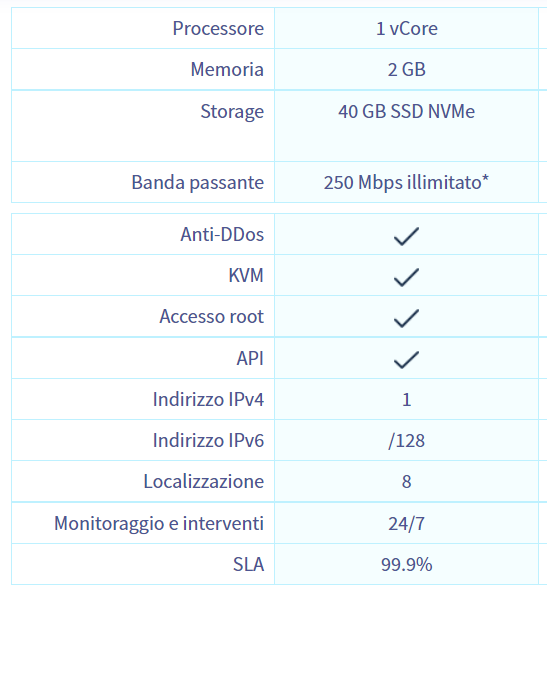
\includegraphics[scale=0.6]{immagini/specifiche_ovh_essential.png}
	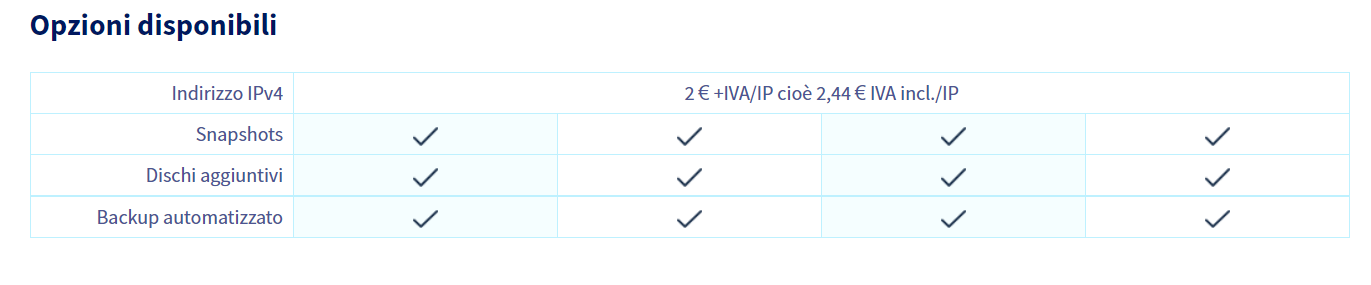
\includegraphics[scale=0.5]{immagini/opzioni_ovh_essential.png}
	\caption{Caratteristiche e opzioni agguntive disponibili della soluzione VPS acquistata
		(\href{https://www.ovhcloud.com/it/vps/compare/}{link})}
	\label{fig:caratteristiche_vps}
\end{figure}
Di seguito (Figura \ref{fig:caratteristiche_vps}) sono riepilogate le principali caratteristiche del servizio acquistato.
Tra le feature incluse spicca la banda passante al VPS, che è garantita e si riferisce alla velocità di trasmissione minima assegnata, inoltre è incluso il sistema di protezione \textit{anti-DDoS OVHcloud}.\hfill\break Una vasta gamma di sistemi operativi sono equipaggiabili per la macchina virtuale, quali Windows Server, Debian, Fedora, CentOS ed Ubuntu, in particolare si è scelto di adottare \textbf{Ubuntu 16.04 LTS}. Inoltre è da sottolineare che il \textit{Service Level Agreement} per il servizio scelto è caratterizzato da un tasso di disponibilità mensile pari al 99,9\%.\hfill\break
Una volta finalizzato il pagamento, viene fornito l'accesso alla dashboard principale del servizio scelto tramite lo spazio utente (Figura \ref{fig:dashboard_vps}).
\begin{figure}[ht]
	\centering
	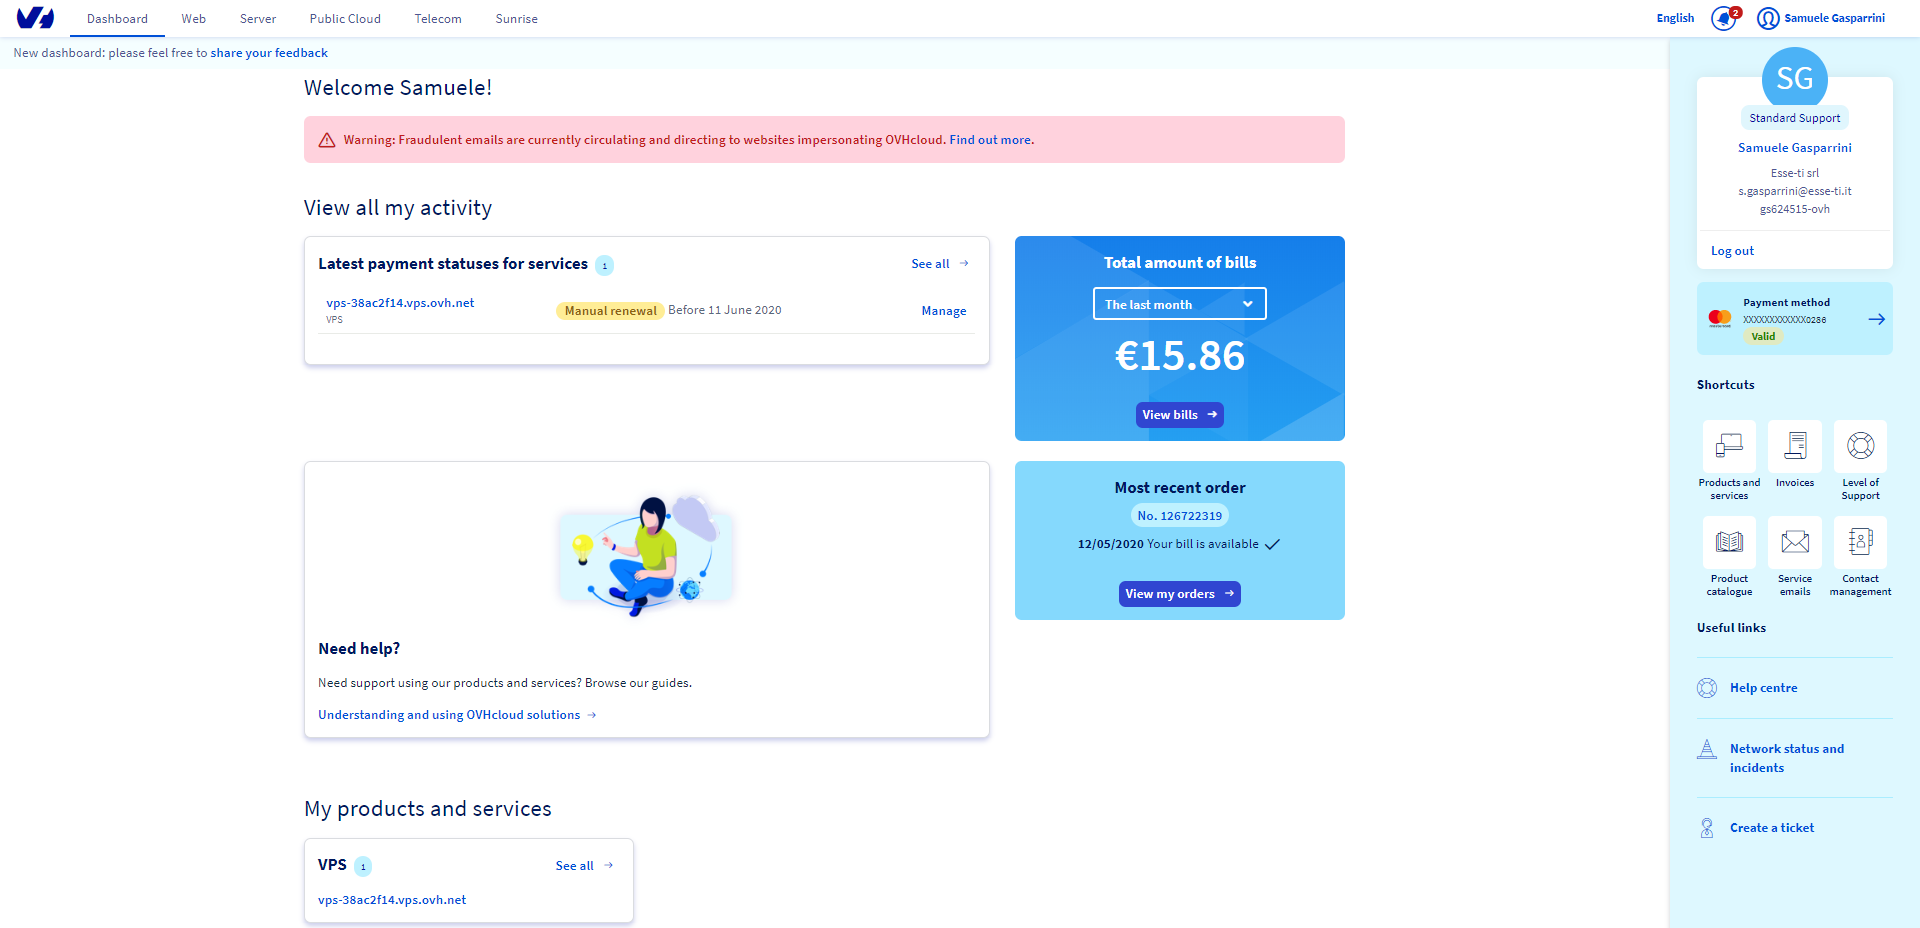
\includegraphics[width=1\textwidth]{immagini/img9.png}
	\caption{Dashboard OVHCloud}
	\label{fig:dashboard_vps}
\end{figure}
Da qui, è possibile accedere al servizio acquistato direttamente con un \textit{click} nella sezione server, ma anche alle ultime fatture pagate, nonchè andare a gestire tutto ciò che riguarda l’account utente con il pannello sulla destra della schermata.
A partire dalla dashboard si individuano due aree diverse, una per la gestione del nostro account e le informazioni personali, l’altra per la gestione dei servizi acquistati. La dashboard per la gestione delle informazioni personali dell’utente permette di scaricare le fatture dei pagamenti effettuati i servizi attivi, con lo stato di funzionamento, e la modalità di rinnovo (manuale o automatica), inoltre è possibile modificare, aggiungere e rimuovere i metodi di pagamento ed infine di aprire e gestire eventuali ticket, sia per assistenza tecnica che assistenza commerciale, con i relativi contatti di supporto.
Per quanto riguarda invece la gestione dei servizi acquistati come appunto VPS, server dedicati ecc., possiamo accedere, a partire dalla dashboard principale sotto la voce \textit{My product and services}, ad un pannello di controllo generale dove è possibile selezionare quale prodotto, tra quelli acquistati, andare a gestire. Possiamo fare click direttamente sull’hostname della VPS acquistata e verremo reindirizzati al pannello di riepilogo (Figura \ref{fig:pannello_di_controllo_vps}).
\begin{figure}[ht]
	\centering
	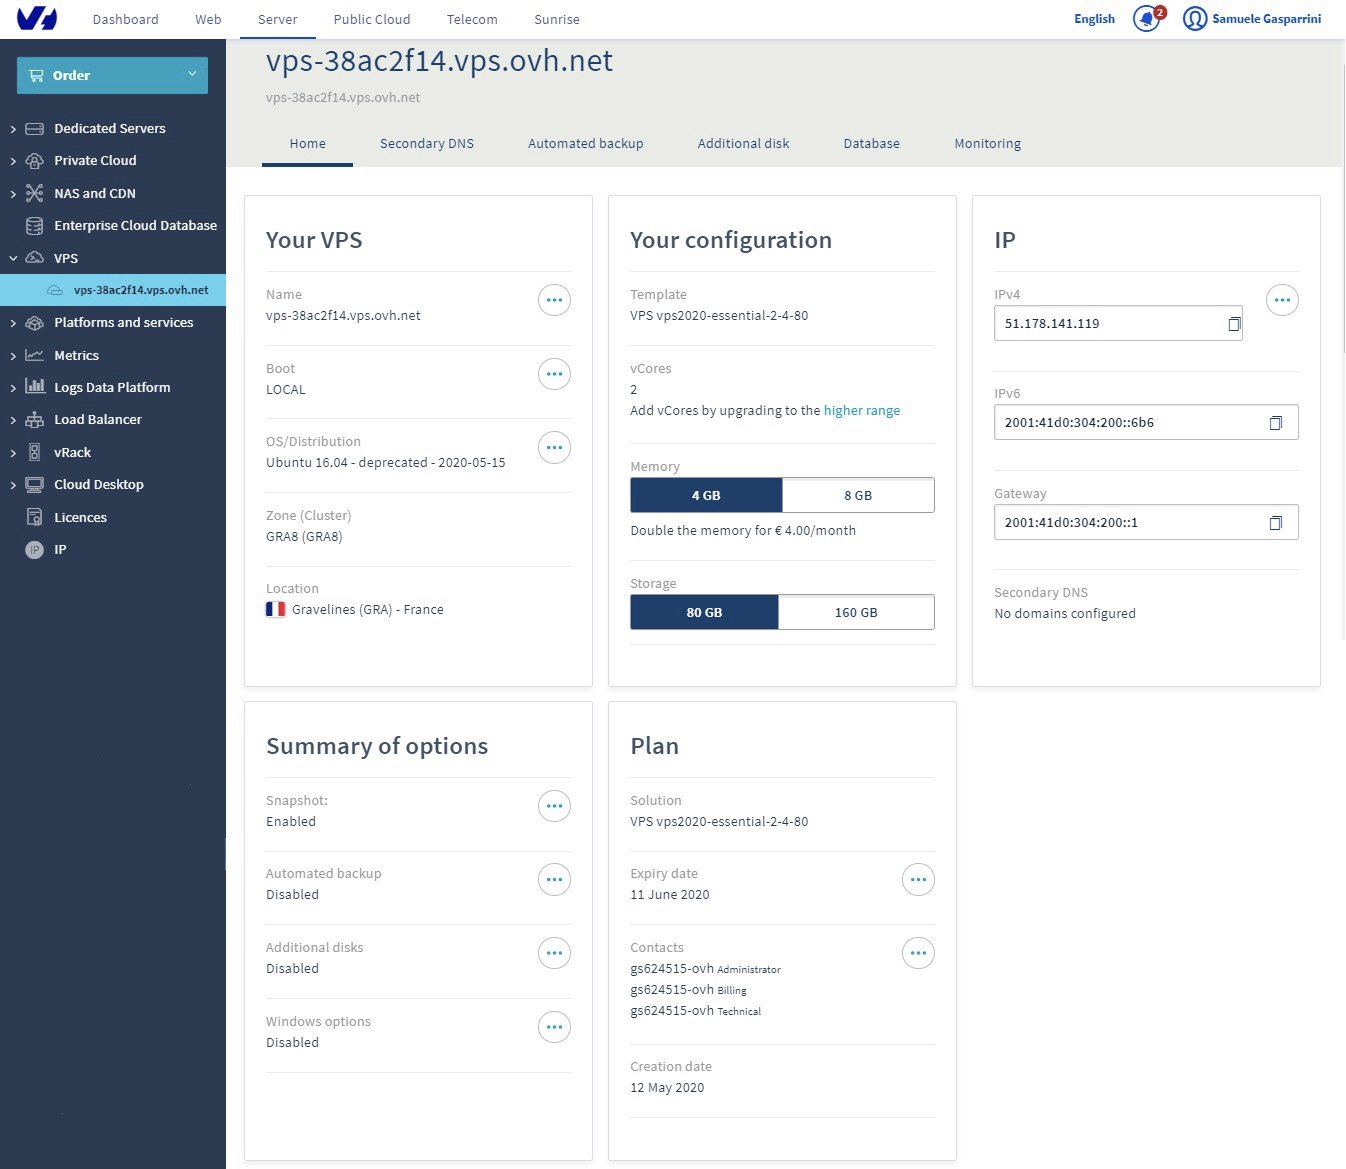
\includegraphics[width=0.6\textwidth]{immagini/pannello_di_controllo_VPS.jpg}
	\caption{Pannello di controllo del servizio VPS acquistato}
	\label{fig:pannello_di_controllo_vps}
\end{figure}

Esso presenta tutte le informazioni di cui possiamo aver bisogno per la gestione della nostra macchina virtuale, in particolare:
\begin{itemize}
	\item informazioni sul sistema operativo;
	\item localizzazione fisica della \textit{server farm} presso cui la VPS è installata;
	\item l'indirizzo IP attraverso il quale è possibile accede alla macchina remota tramite il protocollo sicuro SSH;
	\item un riepilogo delle opzioni attivate o disattivate che sono state opzionate all’acquisto della macchina, così come il piano attuale.
\end{itemize}
Come già evidenziato, con un paio di \textit{click} è possibile fornire più risorse hardware, in termini di RAM o storage, alla nostra VPS, è inoltre possibile  aumentare il numero di unità elaborative passando ad una VPS di livello superiore.

\section{Caratteristiche del gateway adottato dall'azienda }\label{caratteristiche_gateway}

L'azienda Esse-ti S.r.l. ha fornito due gateway con funzionalità di router identici, modello \textit{4G.Router} (Figura \ref{fig:router}), ognuno corredato di una SIM per la connessione all'operatore radiomobile partner. Il modello in questione offre  connettività Internet e consente il telecontrollo dei dispositivi connessi via Wi-Fi, porta LAN o porta seriale.
\begin{figure}[ht]
	\centering
	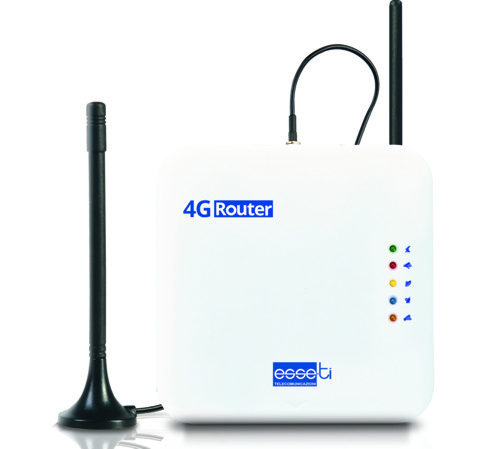
\includegraphics[scale=0.4]{immagini/router_esse_ti.jpg}
	\caption{Gateway 4G.Router fornito ai clienti Esse-ti
		(\href{https://www.esse-ti.it/4g-router}{link})}
	\label{fig:router}
\end{figure}
Ad oggi l'azienda impiega questo dispositivo nel panorama dell'IoT applicato al settore dell'elevazione, con funzionalità che spaziano in molti ambiti per garantire la massima flessibilità d'impiego:
\begin{itemize}
	\item Access Point wireless per offrire connettività Internet Wi-Fi a dispositivi wireless;
	\item Client Dynamic DNS per consentire all’utente di raggiungere da remoto, tramite Internet, il router stesso e tutti i dispositivi connessi via Wi-Fi o porta LAN;
	\item Trasmissione dati in standard RS-232/RS-485/CAN-bus per consentire all’utente di monitorare da remoto, tramite servizio COMNet, i dispositivi connessi alla porta seriale, oppure per consentire ai dispositivi connessi alla porta seriale di inviare automaticamente dati, segnalazioni, notifiche tramite servizio COMNet;
	\item Gateway telefonico per consentire l’invio e la ricezione di chiamate attraverso la rete 4G LTE/UMTS/GSM a telefoni fissi, combinatori o altri dispositivi telefonici collegati all’ingresso FXS, con la possibilità di visualizzare l'identificativo del chiamate;
	\item Gestione servizio roaming;
	\item Ingressi digitali programmabili, configurabili anche con antifurti tecnologici;
	\item Uscite relè attivabili localmente o via SMS, possono anche segnalare eventi come la mancata alimentazione e l'assenza di segnale radiomobile;
	\item Programmazione locale o remota del gateway telefonico tramite telefono (toni DTMF) o via SMS;
	\item Lettura programmazione via SMS;
	\item Invio di segnalazioni ed avvisi tecnici tramite SMS per il controllo della scandenza della scheda SIM, stato della batteria e dell'alimentazione esterna;
	\item Batterie interne di backup per garantire il funzionamento anche in assenza di alimentazione;
	\item Aggiornamento firmare \textit{over-the-air}.
\end{itemize}

Le caratteristiche hardware del gateway includono:
\begin{itemize}
	\item Modulo LTE Cat 1 Penta-Band / UMTS HSPA+ Dual-Band / GSM Dual-Band
	\item Frequenze LTE (700/800/900/1800/2100 MHz) / UMTS HSPA+ (900/2100 MHz) / GSM (900/1800 MHz);
	\item Velocità LTE Cat 1, download max. 10,2 Mbps / upload max. 5,2 Mbps;
	\item Wi-Fi 2.4 GHz - IEEE 802.11b/g/n con supporto ai protocolli di sicurezza WEP, WPA, WPA2, WPA-WPA2, WPA-WPA2-AES;
	\item Dotazione di ingressi e uscite:
	      \begin{itemize}
		      \item Porta LAN con ingresso RJ45 10/100 Mbps;
		      \item Porta FXS (morsetto);
		      \item Morsettiera per trasmissione dati in standard RS-232, RS-485 e CAN-bus;
		      \item Due Uscite relè (NA e NA/NC; 1 A 24 V);
		      \item Due Ingressi optoisolati per allarmi tecnologici;
		      \item Porta micro USB A/B per connessione a pc;
		      \item Alloggiamento SIM Card;
		      \item Connettore antenne esterne SMA.
	      \end{itemize}
	\item Molteplici LED di segnalazione per stato del dispositivo, trasmissione dati COMNet, stato dell'alimentazione, livello del segnale radiomobile ricevuto, stato della linea telefonica connessa alla porta FXS;
	\item Alimentazione  da 11 a 26 Vdc con apposito morsetto o tramite jack per alimentatore esterno 100-240 Vac;
	\item Batteria di backup a tecnologia Ni-MH con capacità di 800mAh a 7,2V che garantisce fino a 8 ore di funzionamento in stand-by o 2 ore di funzionamento attivo.
\end{itemize}
%   - stack iso / osi -> cos'e' un'ip
%   - openvpn
%   - openwrt




\chapter{Overview dell'architettura e delle componenti utilizzate}
\setlength{\parskip}{1em}
\setlength{\parindent}{0em}
\renewcommand{\baselinestretch}{1.15}

\label{ch:overview}

\section{Obbiettivo da ottenere}

In una collaborazione tra il Dipartimento di Ingegneria dell'Informazione e l'azienda \textbf{Esse-ti S.R.L.} ci \`e stato esposto un progetto che consiste nel:

%todo non mi piace come sta messo
\begin{itemize}
	\item fornire a dei clienti un router 4G, su cui possono essere connessi vari dispositivi, ad es. di tipo domotico.
	\item rendere questi dispositivi accessibili ai clienti attraverso internet
\end{itemize}

\begin{figure}[ht]
	\centering
	\includesvg[width=250px]{immagini/diag-goal}
	\caption{Schema concettuale dell'obbiettivo da raggiungere. \cite{icons}}

	\label{fig:schema_concettuale}

\end{figure}

Data la presenza del CG-NAT si vede subito che non \`e realizzabile a meno che il cliente non abbia un'IP pubblico e la sua macchina venga configurata opportunamente. Questo per\`o non \`e possibile nel caso generale, quindi per risolvere efficacemente questa topologia si deve necessariamente introdurre una terza macchina provvista di IP pubblico e che funga da ponte tra il 4G.Router e il cliente.


\begin{figure}[ht]
	\centering
	\includesvg[width=250px]{immagini/diag-real}
	\caption{Schema concettuale dell'architettura che si dovr\`a implementare. \cite{icons}}

	\label{fig:schem_architettura_reale}

\end{figure}

%todo rivedi frase
In questo modo si pu\`o configurare una VPN sul server OVH e connettervi sia il 4G.Router che la macchina del cliente. In questo modo l'unica configurazione che il cliente dovr\`a fare \`e l'installazione di un cliente VPN, ci\`o \`e il minimo possibile di configurazione.

La configurazione virtuale vista dal 4G.Router e dai clienti sar\`a quindi:

\begin{figure}[ht]
	\centering
	\includesvg[width=250px]{immagini/diag-virtual}
	\caption{Topologia virtuale. \cite{icons}}

	\label{fig:schema_architettura_virtuale}

\end{figure}


\section{Specifiche dei componenti}

i componenti necessari sono:

\begin{itemize}
	\item Esse-ti 4G.Router
	\item Server
	\item Host domotico
	\item Macchina del cliente
\end{itemize}

vediamo le caratteristiche minime che i componenti dovranno avere:

\subsubsection{Esse-ti 4G.Router}

Ci \`e stato fornito dall'azienda Esse-ti, consiste in un gateway 4G con funzionalità di router. Le specifiche complete possono essere trovate sul sito del produttore (\href{https://www.esse-ti.it/4g-router}{link})


\begin{figure}[ht]
	\centering
	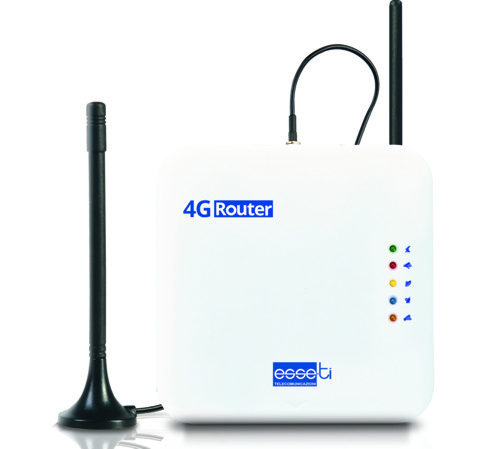
\includegraphics[width=250px]{immagini/4grouter.jpg}
	\caption{4G.Router}

	\label{fig:esse-ti-router-4g}

\end{figure}

Per l'implementazione di questa architettura sono necessarie solo un sub-set delle specifiche:

\begin{itemize} %TODO e' copiato e incollato va sistemato
	\item Access Point wireless per offrire connettività Internet Wi-Fi a dispositivi wireless
	\item Client Dynamic DNS per consentire all’utente di raggiungere da remoto, tramite Internet, il router stesso e tutti i dispositivi connessi via Wi-Fi o porta LAN
	\item Gateway telefonico per consentire l’invio e la ricezione di chiamate attraverso la rete 4G LTE/UMTS/GSM a telefoni fissi, combinatori o altri dispositivi telefonici collegati all’ingresso FXS
\end{itemize}

Presenta inoltre come sistema operativo una versione personalizzata di OpenWrt.

La configurazione del dispositivo puo' essere fatta sia da terminale, entrando in ssh, sia da interfaccia web:

\begin{figure}

	\newlength{\tempheight}
    \setlength{\tempheight}{23ex}

	\centering%
    \begin{subfigure}[t]{0.5\textwidth}
        \centering%
        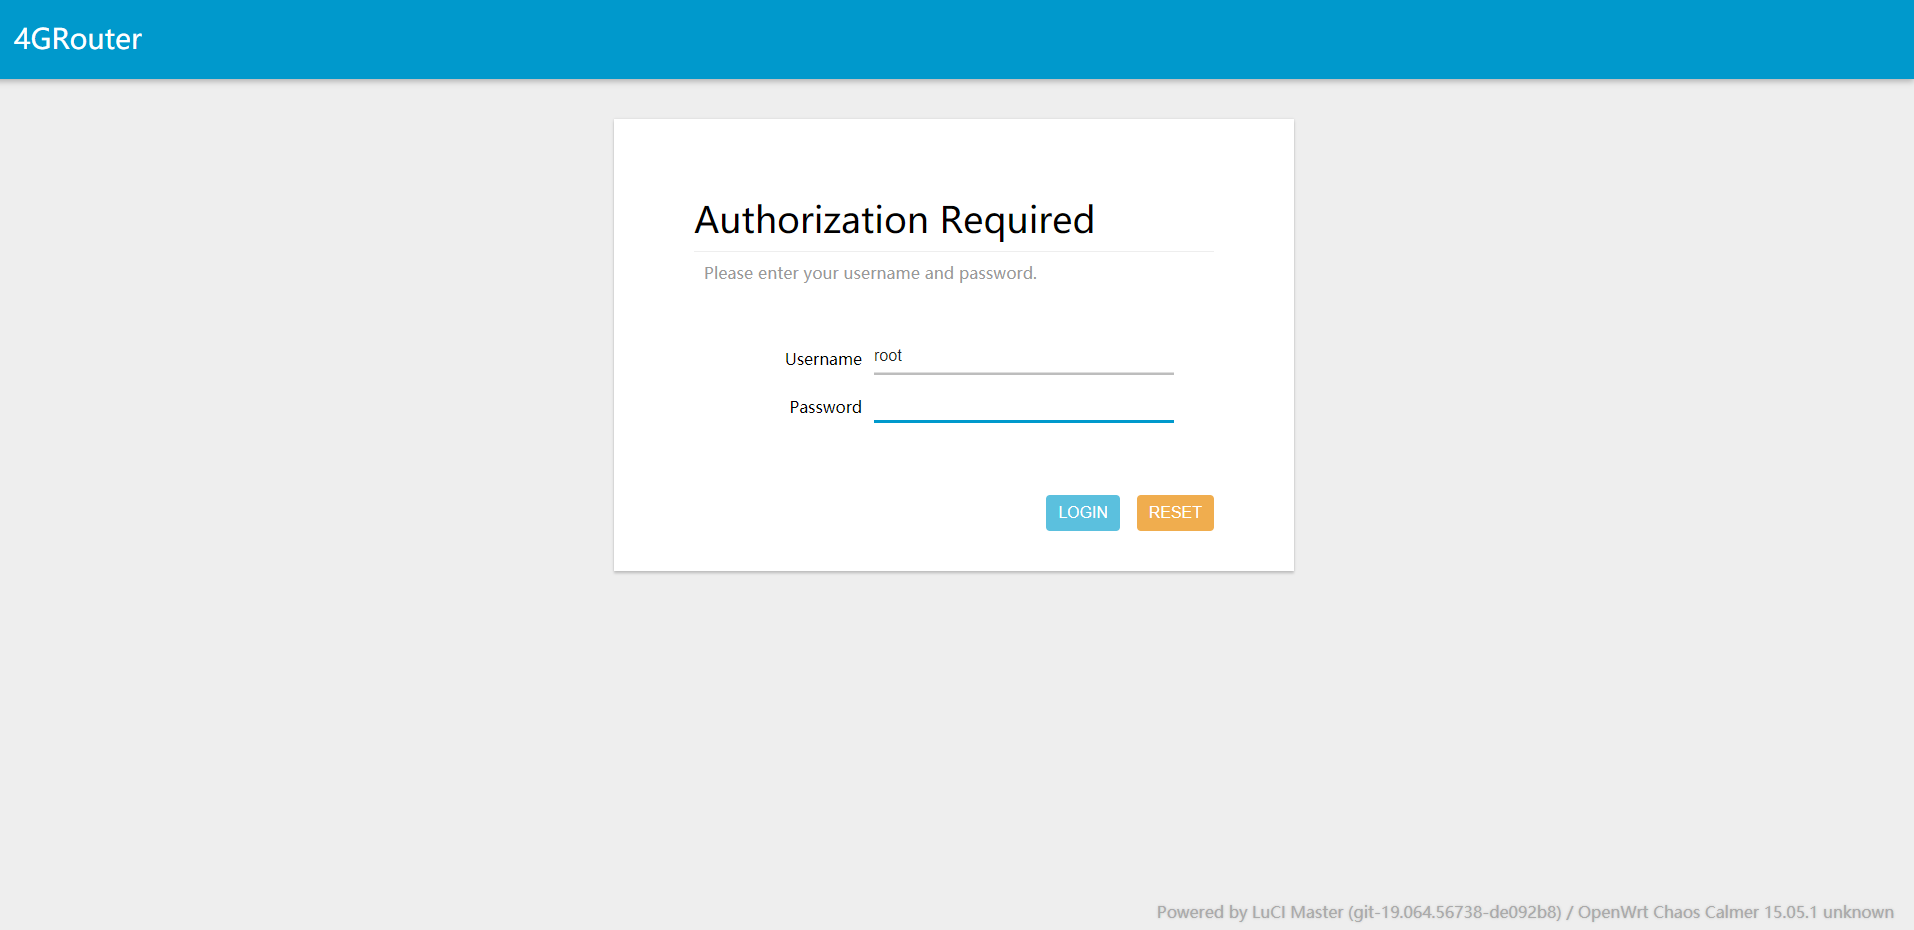
\includegraphics[totalheight = \tempheight]{immagini/interfacciar4g_init.png}
        \caption{Schermata di autenticazione}
    \end{subfigure}%
	\hfill
    \begin{subfigure}[t]{0.5\textwidth}
        \centering%
        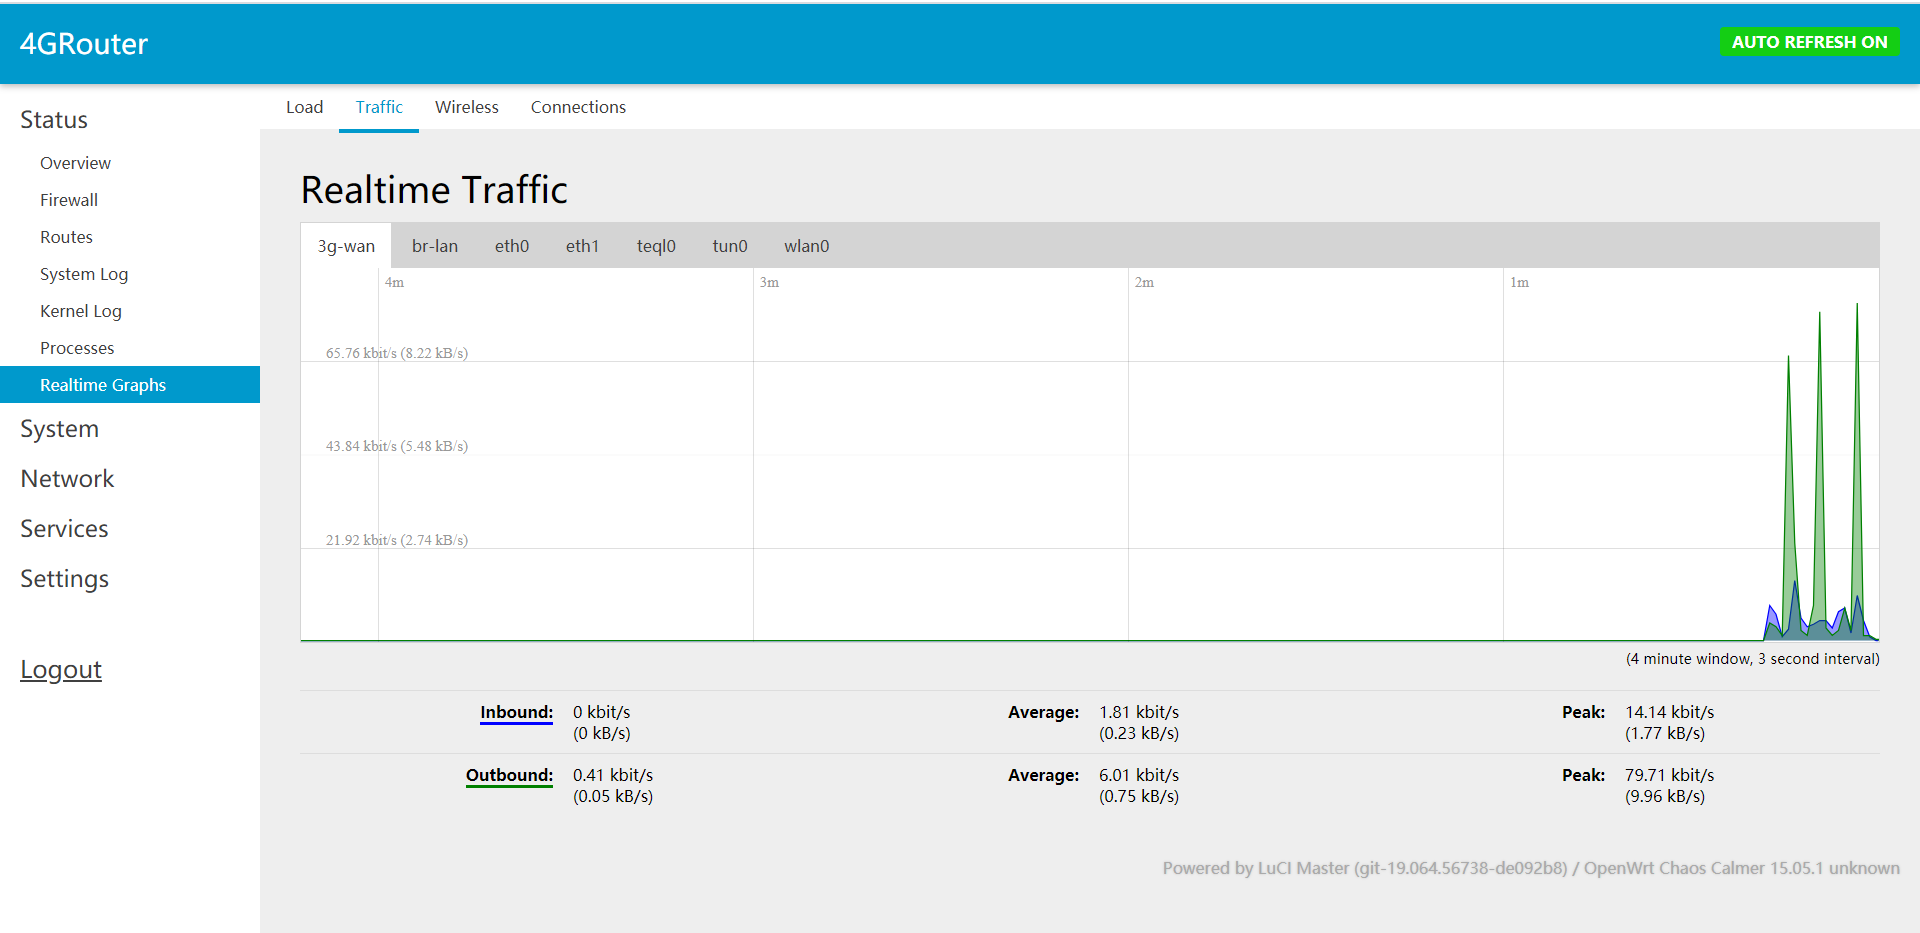
\includegraphics[totalheight = \tempheight]{immagini/interfacciar4g_traffic.png}
        \caption{Grafico del traffico}
    \end{subfigure}

	\vspace{1ex}

	\begin{subfigure}[b]{\textwidth}
        \centering%
        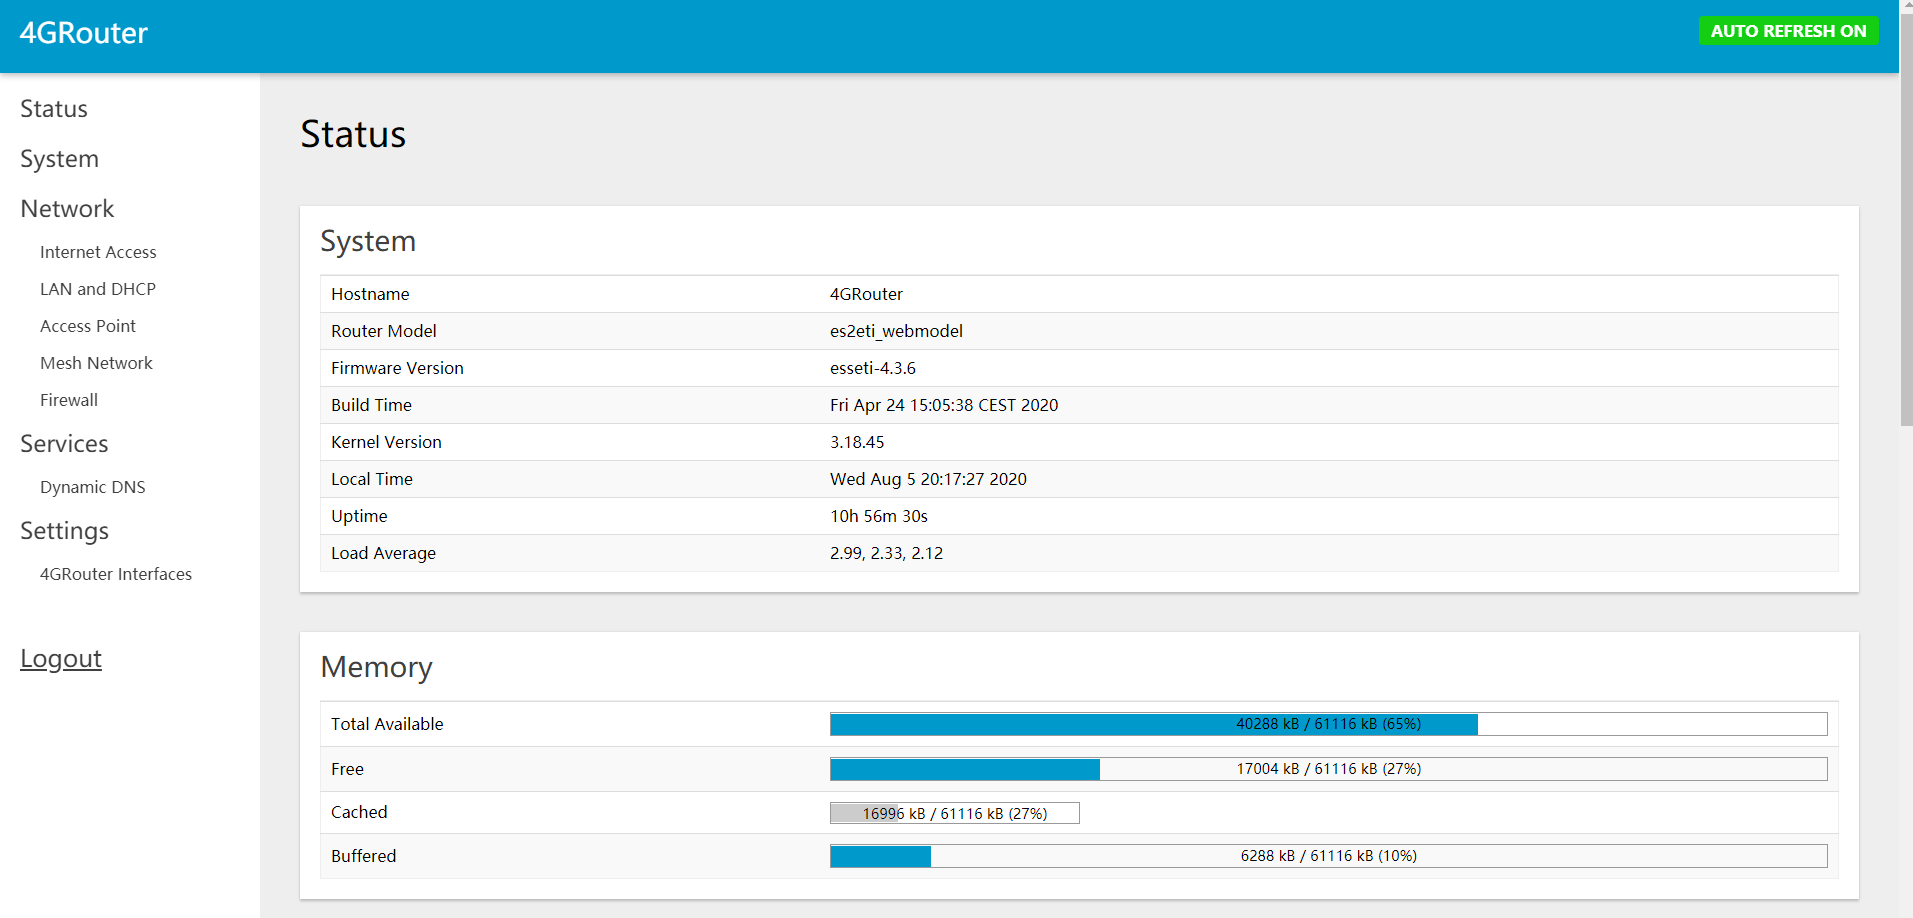
\includegraphics[totalheight = 1.6\tempheight]{immagini/interfacciar4g_status.png}
        \caption{Schermata con stato riassuntivo}
    \end{subfigure}

\end{figure}

L'interfaccia web e' una versione personalizzata di \href{https://openwrt.org/docs/guide-user/luci/start}{Luci}.

Per semplicita' si fara' riferimento all'\textit{Esse-ti 4G.Router} chiamandolo semplicemente router.

\subsubsection{VPS OVHCloud}

La VPS ha il solo vincolo di dover avere un'ip pubblico e una connessione a internet abbastanza veloce. Dovra' infatti sopportare un traffico simmetrico in upload / download.

Per la realizzazione della topologia e' stata selezionata una macchina una VPS del provider OVHCloud, con le seguenti caratteristiche:

\begin{itemize}
	\item 2 core virtuali
	\item 4Gb di memoria ram
	\item 80Gb di storage NVMe
	\item 500Mbps simmetrici di banda
	\item ipv4 pubblico
	\item Ubuntu 16.04
\end{itemize}

Per semplicita' si fara' riferimento alla \textit{VPS OVHCloud} come server.

\subsubsection{Host domotico}

%TODO don't like
Per effettuare le varie operazioni di testing e' stato aggiunta \it{raspberry pi} che ha svolto il ruolo di "host domotico". Sono state fatti test con ping e iperf per testare che tutta la topologia sia stata configurata correttamente.


\subsubsection{Macchina del cliente}

%TODO da espandere
Deve poter essere una qualunque macchina, non ha vincoli di sistema operativo

Necessita di avere il client openvpn installato:

\begin{itemize}
	\item con sistema operativo Windows si deve scaricare l'eseguibile dal \href{https://openvpn.net/client-connect-vpn-for-windows/}{sito ufficiale}
	\item su linux e' sufficiente cercare nei repository ufficiali della distribuzione che si sta usando.
\end{itemize}



% overview
%   - overview dell'architettura da ottenere
%   - specifiche dei componenti (chi deve avere un'ip pubblico, chi deve avere 0 config etc)


%\input{contenuti/capitolo_2}
% server
%   - ca e chiavi varie
%   - installazione e config di openvpn
%   - test della config con singolo host
%   - automazione creazione delle config

%\input{contenuti/capitolo_3}
% router
%   - configurazione openwrt
%   - configurazione firewall

%\input{contenuti/capitolo_4}
% testing della config
%   - test di connessione tra router e server
%   - test di connessione tra router e host vpn
%   - test della connessione tra host sotto il router e host della vpn

%\input{contenuti/capitolo_5}
% multi-istanza
%   - multi-istanza openvpn
%   - problemi di sicurezza relativi

%\input{contenuti/capitolo_6}
%   - multi-istanza con virtualizzazione del server su docker

%\input{contenuti/conclusione}


%___________BIBLIOGRAFIA____________________

\newpage

\thispagestyle{empty}


\begin{thebibliography}{a}

\item \url{https://info.support.huawei.com/network/imagelib/getImagePartList?product_family=Router&product_type=Access%20Router%7CIOT%20Gateway&domain=&lang=en}

\end{thebibliography}


%___________________________________________________________

%\input{contenuti/ringraziamenti}

\end{document}